\chapter{Hardware Subsystems}
\label{chap:hardware_subsystems}
In this chapter building blocks of the proposed system, each of which were separately prototyped to allow a good degree of parallelisation, are described. The driver software that makes each unit functional is also mentioned. We discuss the top-level software that brings these blocks together into a functional system in the chapter \ref{chap:system_software}.

\section{Monitoring Device}
The monitoring device is designed to be a simple device that acquires data from the sensors, stores the data and sends it to the base station when the ZigBee link is available. It contains a microcontroller, a set of sensors for data acquisition, a memory card to store data and a ZigBee module for wireless communications.

\begin{figure}[htb]
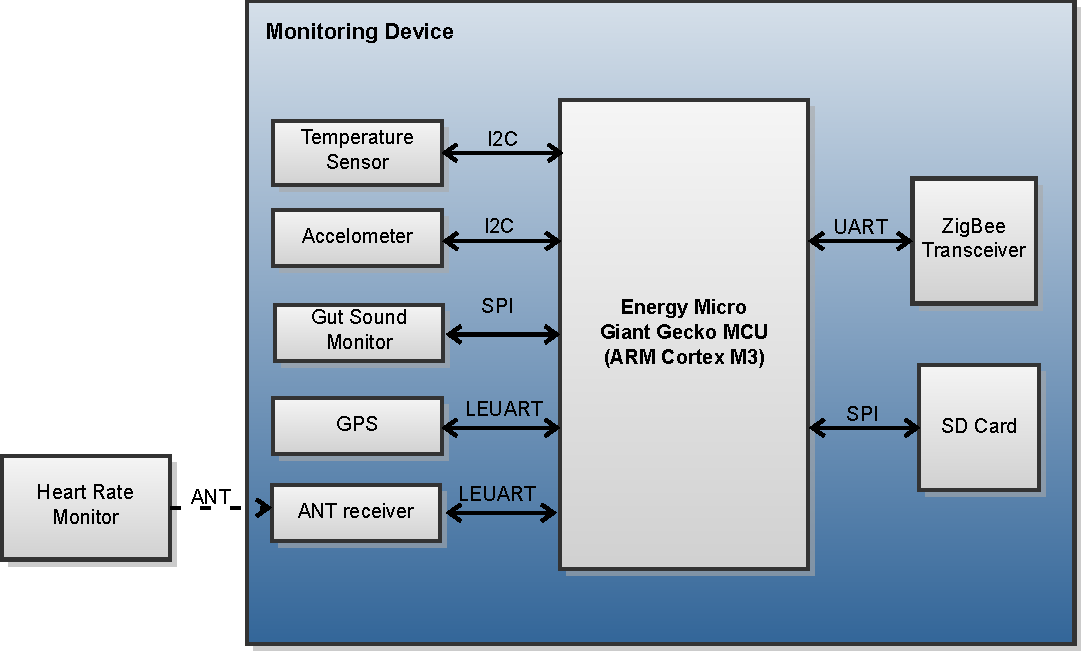
\includegraphics[width=\textwidth]{Images/MonitoringDeviceBlockDiagram}
\caption{Block Diagram: Monitoring Device}
\label{fig:monitoring_device_block}
\end{figure}

The following sub-chapters will discuss the implementation of each subcomponent of the monitoring device, shown in Figure \ref{fig:monitoring_device_block}, together with the properties of the hardware and how they map to the requirements of the project.


\subsection{The Microcontroller (MCU)}
As the monitoring device is required to be a battery-operated system that contain a number of diverse peripherals, choosing the right central processing unit was essential. Reviewing existing microcontrollers in the market we opted for an EFM32 Giant Gecko microcontroller from Energy Micro, which contains a 32-bit ARM Cortex M3 core and a set of on-chip peripheral interfaces. The EFM32 was considered to be a good match for the requirements, as shown in the table \ref{tab:microcontroller_properties}.

\begin{table}[htb]
\begin{tabular}{|m{0.45\textwidth}|m{0.45\textwidth}|}
\hline 
	\textbf{Device Properties} & 
	\textbf{Corresponding Requirements} \\ 
\hline
	\phantom{.}
	\begin{itemize}
	\item up to 48 MHz high-frequency operation
	\end{itemize}&
	\phantom{.}
	\begin{itemize}
	\item handle large data volumes from multiple sensors and audio
	\end{itemize} \\	
\hline
	\phantom{.}
	\begin{itemize}
	\item different levels of sleep
	\item fast wake up time (2 $\mu S$)
	\item 32.768 kHz low-frequency operation for sleep modes
	\item low energy periphals operational even in deep sleep modes
	\item DMA and PRS (Peripheral Reflex System) for acquiring data without waking up the processor core
	\end{itemize} &
	\begin{itemize}
	\item long battery life
	\item long periods of sleep
	\item low energy periodic sampling
	\end{itemize} \\
\hline
	\phantom{.}
	\begin{itemize}
	\item 128 KB SRAM, 1MB flash memory
	\end{itemize} &
	\phantom{.}
	\begin{itemize}
	\item ease of development
	\item suitable for overheads introduces by C++
	\end{itemize} \\
\hline
	\phantom{.}
	\begin{itemize}
	\item 3 x USART with I2S support
	\item 2 x low energy UART (LEUART)
	\item 2 x I2C interfaces
	\end{itemize} &
	\phantom{.}
	\begin{itemize}
	\item various interfaces for peripherals and sensors
	\end{itemize} \\
\hline
	\phantom{.}
	\begin{itemize}
	\item 64-pin TQFP package
	\end{itemize} &
	\phantom{.}
	\begin{itemize}
	\item ease of soldering (lack of BGA mounting equipment)
	\end{itemize} \\
\hline 
\end{tabular} 
\caption{Microcontroller properties}
\label{tab:microcontroller_properties}
\end{table}

Some of the more specialized properties of the microcontroller which give it advantages for our solution are briefly explained below:

\subsubsection*{Energy Modes and Low Energy Peripherals} The EFM32 microcontrollers offer four levels of sleep, and some special peripherals (called low energy or LE peripherals) that are able to keep functioning even in deep sleep modes. Of particular interest to us are the LEUART interface which while deeper sleep modes provide more energy savings, it also becomes more difficult to implement a reasonable level of active functionality. An overview of sleep modes and available peripherals in each is presented in table \ref{tab:microcontroller_modes}.

\begin{table}[htb]
\centering
\begin{tabular}{|l|l|m{6cm}|}
\hline
	\textbf{Energy Mode}&
	\textbf{Power consumption}&
	\textbf{Description}  \\ 
\hline
	EM0 &
	$200 \frac{\mu A}{MHz}$ &
	All peripherals active, CPU core active  \\ 
\hline
	EM1 &
	$50 \frac{\mu A}{MHz}$  &
	All peripherals active, CPU core sleep  \\ 
\hline
	EM2 &
	$1.2 \mu A$  &
	LEUART, LETIMER, I2C, RTC, LCD, PCNT, LESENSE, ACMP, OPAMP, USB active  \\ 
\hline
	EM3 &
	$0.9 \mu A$  &
	Full CPU and RAM retention, asynchronous external interrupts and I2C can wake up the device   \\ 
\hline
	EM4 &
	$20 nA$  &
	All functionality off, GPIO pin retention and wake up from GPIO interrupt  \\ 
\hline 
\end{tabular} 
\caption{Microcontroller energy modes}
\label{tab:microcontroller_modes}
\end{table}

\subsubsection*{Direct Memory Access (DMA)} DMA allows blocks of data to be moved between RAM and peripherals without CPU intervention, thus freeing CPU resources and allowing longer periods of sleep, as well as offering stable high bandwidth memory transfers for operations like audio acquisition.

Further details of how the PRS, DMA and different sleep modes are used in the system is provided in chapter \ref{chap:system_software}


\subsection{Heart Rate Monitor (HRM)}
The heart rate is an important vital sign for any health monitor, although designing a portable device to acquire heart rate is not a trivial task. The issues of electrode placement, filtering out changes due to subject movement and processing the resulting ECG signal are challenging and time consuming. Another challenge specific to our project is acquiring both gut sounds and the heart rate; it is not possible to reliably acquire both signals from the same physical location so a wired microphone or electrode would have to be attached to the horse. 

To address both these problems, we chose an ANT wireless module (ANTAP281M4IB from Nordic Semiconductor / Dynastream) that can be used with any ANT+ compatible heart rate chest strap, commercially available for both horses and humans. Attaching a separate heart rate monitor chest strap and transmitting heart rate information wirelessly solves the problems mentioned above and brings the additional advantage of making the system usable for humans.


\begin{table}[htb]
\centering
\begin{tabular}{|m{0.45\textwidth}|m{0.45\textwidth}|}
\hline 
	\textbf{Device Properties} &
	\textbf{Corresponding Requirements}  \\ 
\hline
	low power  
	\begin{itemize}
	\item peak rx current 17mA
	\item peak tx current 15mA
	\item idle (no RF activity) current 2$\mu A$
	\item search current 2.8mA
	\end{itemize}
	automatically enter idle mode if no activity detected
	&
	low energy periodic sampling  \\ 
\hline
	simple UART interface &
	ease of development \\
\hline
	can pair with a particular ANT+ HRM chest strap &
	monitoring multiple horses \\
\hline 
\end{tabular} 
\caption{ANT HRM interface properties}
\label{tab:ant_properties}
\end{table}

\textbf{Interface:}
The ANT module handles most RF processing internally and offers a simple UART interface to the microcontroller with configurable baud rate. Since there message volume passed between the ANT and the EFM32 will be relatively small (less than a hundred bytes per message, and a message rate of 1-4 Hz while active) and because the messages can arrive asynchronously while the monitoring device is in sleep mode, a LEUART port with a baud rate of 4800 was used for the ANT module connection.


\textbf{Driver:}
The ANT driver, whose implementation is based on the ANT+ HRM receiver example from Dynastream, can be described as consisting of three layers:

\begin{description}
\item{\bfseries Message reception and format validation layer:} 
The LEUART port, which is able to receive data even while the EFM32 is sleeping in EM2, sends the characters to the ANT driver which validates the correctness of the received ANT messages according to the ANT message structure\footnote{\url{ http://www.thisisant.com/resources/ant-message-protocol-and-usage/}}.  Validated messages are passed to the ANT protocol layer for handling. Similarly, data received from the ANT protocol layer is packaged according to the ANT message format and put through the LEUART port.

\item{\bfseries ANT Protocol layer:}
This layer handles details of the ANT protocol such as configuring the RF channels and network key, and is largely based on the Dynastream standard  implementation. One important function is handling disconnections and device pairing. The current behaviour is to pair with the particular HRM chest strap as soon as a connection is made, and attempt to reconnect to the same device if disconnected. ANT+ specific messages are passed to the ANT+ layer and actual message sending/receiving happens through the interfaces to the message layer.

\item{\bfseries ANT+ HRM protocol handling:}
This layer handles the ANT+ data pages received from the heart rate monitor chest strap, which contain a variety of information about the monitored heart rate. Our current implementation only reads the computed heart rate in beats per minute and makes this data available through the standard Sensor interface. Please consult the ANT+ Heart Rate Monitor device profile document\footnote{\url{http://www.thisisant.com/resources/heart-rate-monitor/}} for more information.
\end{description}


\subsection{Temperature Sensor}

As with many other warm-blooded animals, body temperature can be a valuable tool for diagnosis in horses. While electronic temperature measurements are usually done by an element that comes into physical contact with the subject, doing temperature measurements in this manner on a moving horse is likely to cause fluctuations in the read values. This is the reason we preferred to use a contactless temperature sensor for our implementation. 

TMP006\footnote{\url{http://www.ti.com/lit/ds/symlink/tmp006.pdf}} which is a contactless infrared temperature sensor from Texas Instruments was chosen for the project. 


\begin{table}[htb]
\centering
\begin{tabular}{|m{0.45\textwidth}|m{0.45\textwidth}|}
\hline 
	\textbf{Device Properties} &
	\textbf{Corresponding Requirements}  \\ 
\hline
	low power:
	\begin{itemize}
	\item 240-325 $\mu A$ during active conversion
	\item 90 $\mu A$ in sleep mode 
	\end{itemize}  &
	low energy periodic sampling  \\ 
\hline
	contactless temperature measurement &
	portable, mobile monitoring device \\
\hline
	passive (slave) device over I2C bus &
	advantageous for a system with lots of sensors, will not send and generate interrupts unless requested \\
\hline 
\end{tabular} 
\caption{Temperature Sensor properties}
\label{tab:temp_sensor_properties}
\end{table}

\textbf{Interface:} The TMP006 offers an SMBus-compatible interface, which is interoperable with I2C and was connected to the I2C interface on the microcontroller. Controlling device functionality and accessing measurement data is done via "write to register" and "read from register" commands. 

\textbf{Driver:} Our TMP006 driver configures device sleep state and conversion rate by writing values to the appropriate registers. The temperature measurement is provided by reading the two registers which contain the voltage generated by the thermopile and the die temperature. The temperature of the object can be calculated from these two data. However this calculation involves heavy floating point arithmetic and it is rather inefficient on the microcontroller. Therefore, the "raw" temperature reading consisting of these two values is not processed on the monitoring device any further but sent to the base station, whose ARM11 core is much more efficient at handling this calculation. 


\subsection{GPS}
A popular peripheral in many consumer devices today, GPS (Global Positioning System) allows tracking the position of a sensor in terms of global coordinates. While not immediately useful for clinical purposes, the ability to track the location of horses on this level can be beneficial if recording of movements or activity recognition \TODO{REF:}  [High Classification Rates for Continuous Cow Activity Recognition using Low-cost GPS Positioning Sensors and Standard Machine Learning Techniques.]  is desired over a longer period of time in a larger area (for free-roaming horses or other animals). 

Commercial drop-in GPS modules are available and straightforward to use, but power consumption while searching limits the possibilities for a battery-powered system with energy efficiency focus. We chose a UP500 GPS module from Fastrax \footnote{\url{http://www.fastraxgps.com/products/gpsantennamodules/500series/up500/}}
for our project. UP500 is a GPS receiver module with embedded antenna offered in a very small package, and offers significant power savings by providing an option to save satellite data to RAM while still being able to wake up from this state and get a position fix within a few seconds (called a “hot start”). 

\textbf{Interface:} The UP500 with the microcontroller via UART and uses a baud rate of 9600 (8 data bits, 1 stop bit, no parity). The Low Energy UART (LEUART) peripheral on the EFM32 was used for this connection, which can receive data at low baud rates even while in deep sleep mode (down to EM2).

\textbf{Driver:}
\begin{itemize}
\item{Data acquisition:}
For maximum energy efficient operation, the GPS driver configures the GPS module to use LEUART interface with DMA. DMA transfers incoming NMEA messages into a fixed size buffer when new data is available. The LEUART module is configured to generate an interrupt whenever it receives the newline character (0x0A). Since every NMEA message ends with a newline, an interrupt is generated every time a complete message is received, and the contents of the DMA buffer are copied to another internal buffer for processing at a later time.

\item{Parsing NMEA messages:} \TODO{} simple string parsing, comma delimited fields,NMEA message types GPRMC and GGPA are handled
\begin{itemize}
\item output: valid position fix, latitude and longitude
\end{itemize}

\item{Sleep mode:} The UP500 does not have a dedicated sleep pin, but once satellite data has been acquired it is possible to put the device into a sleep-like mode where the power consumption becomes quite low. This is done by turning off the power to the $V_{cc}$ supply pin, while keeping the $V_{bat}$ supply pin active. By keeping ephemeris data in RAM, the GPS is thus able to establish the position quickly when the $V_{cc}$ supply is reinstated. Switching the $V_{cc}$ supply is done via a transistor attached to a GPIO pin, consult section\ref{sec:pcb_gps} for more details.
\end{itemize}


\subsection{Accelerometer}
In addition to the location tracking capabilities provided by the GPS, it can be useful to measure smaller movements with higher precision. Accelerometer data collected in this manner can be used to detect lameness and injuries. The particular challenge for using an accelerometer in our system was the high sampling rate necessity - the collected acceleration data will not be useful at low sampling rates\footnote{\TODO{find a good citation for this}}. 

While high sampling rate itself is not a problem for the EFM32 microcontroller, it conflicts with low energy periodic sampling - if the microcontroller has to poll the device for new data at a high frequency, it will not have a lot of time to sleep. An accelerometer that contains an on-chip buffer can remedy this problem; the MCU can simply enable sampling, go back to sleep, and wake up when the desired number of samples have been acquired to read them from the sensor's own buffer.

We chose the 3-axis  ADXL350 \footnote{\url{http://www.analog.com/en/mems-sensors/mems-accelerometers/adxl350/products/product.html}} digital accelerometer from Analog Devices for the project. It is capable of measuring acceleration in the ranges ±1g, ±2g, ±4g or ±8g and it has a FIFO buffer which allowed us to implement the scheme discussed in the previous paragraph.

\begin{table}[htb]
\centering
\begin{tabular}{|m{0.45\textwidth}|m{0.45\textwidth}|}
\hline 
	\textbf{Device Properties} &
	\textbf{Corresponding Requirements}  \\ 
\hline
	\phantom{.}
	\begin{itemize}
	\item Ultralow power: $45 \mu A$ in measurement mode and $0.1 \mu A$ in standby mode
	\item FIFO buffer can hold up to 32 samples
	\end{itemize} &
	low energy periodic sampling  \\ 
\hline 
\end{tabular} 
\caption{Accelerometer Sensor properties}
\label{tab:accelerometer_properties}
\end{table}

\textbf{Interface:} Similar to the TMP006, the ADXL350 is interfaced through the I2C bus; controlling device functionality and accessing measurement data is done via "write to register" and "read from register" commands. 

\textbf{Driver:} ADXL350 supports both SPI and I2C interfaces. In this project, it is used in I2C mode. The accelerometer offers a 32-level FIFO which is used in Stream mode, meaning that samples will be continuously accumulated in the FIFO buffer at the desired sampling rate, and old samples will be discarded. Sample rate configuration, sleep and wakeup are all supported through writing to the appropriate registers, which have their own wrapper functions in the driver.
 
\subsection{Gut Sound Monitoring}
One key feature of the desired Equine Health Monitoring System is the possibility to acquire and record sounds coming from horses guts which can come very useful for diagnosis of multiple health disorders in the digestive tract of the animal under observation.

As it was mentioned in chapter \ref{chap:research} listening the gut is a common task performed by a specialist during a regular physical examination. This is done by placing a stethoscope in several parts of the animal's trunk. Intermittent noises that will repeat every 15-30 seconds will be detected in a healthy animal. The specialist will monitor this sounds for an interval of 4-5 minutes. The aim of the designed system is to record and store those sounds which will eliminate the need for a physical examination in situ by a specialist.


\subsubsection{Audio acquisition requirements}
As part of the background research phase it was found that digital recordings of gut noises are regrettably not easily available on the web and despite of different attempts it was not possible to obtain an audio sample of good quality that could be used as a reference. Hence a proper signal profiling and characterization could not be performed. Because of that the audio acquisition system was designed so that it preserves the mayor amount of information present in the original signal and the parameters were selected to fulfill the hearing capabilities of the final human user (a veterinary specialist).

The recording of audio samples implies two major challenges that are not shared by the other sensors in the system.

\begin{description}
\item[Real time constraints:]
In order to acquire an audio stream without distortion accurate periodic sampling must be ensured. That means that during a recording task delays or failures in fetching the samples are inadmissible.

\item[High data rate and memory usage:]
While in the case of other sensors like the temperature sensor and GPS for example fetching a few bytes every 2-3 seconds is enough to provide reliable real-time information, storing an audio stream requires receiving thousands of samples per second. The system capabilities like memory size and bus bandwidth will impose physical barriers to the parameters use for audio sampling.
\end{description}


\subsection{Sampling parameters and component selection justification}
Taking in consideration the requirements as well as the capabilities of the selected system microcontroller platform the audio sampling parameters were set as shown in table \ref{tab:sampling_parameters}. Other audio related projects in this platform were also used as a reference for setting this parameters. 

\begin{table}[htb]
\centering
\begin{tabular}{|l|l|m{4cm}|}
\hline
	\textbf{Parameter} &
	\textbf{Value} &
	\textbf{Justification} \\
\hline
	Sampling frequency &
	8000Hz &
	The microcontroller is not able to handle the recording of higher frequencies.
	Most of the information present in gut sounds is presumed to be in the low frequency range. \\
\hline
	Sample word size &
	16bits &
	High dynamic range. Available in many AD-converters. \\
\hline
	Recording time &
	240 sec &
	To mimic the examination done by a specialist \\
\hline
\end{tabular}
\caption{Audio sampling paramters}
\label{tab:sampling_parameters}
\end{table}

According to that the memory space in bytes required for one single recording can be calculated as follows:
\begin{align*}
\centering
Size_{audio}&=f_{sampling} * \frac{Bits}{Sample}* t_{recording} \\
Size_{audio}&=8000 Hz * 16 \frac{Bits}{Sample}* 240s \\
&= 128kbit/s * 240s \\
&= 3.75MByte
\end{align*}

As it can be noted this is a very high amount of data and thus the use of a external memory device for storage is required as it is explained in section \ref{sec:data_storage}.

\subsection{Component selection justification}
The component ADMP441 from Analog Devices was chosen for the audio acquisition peripheral. This single-chip MEMS (Micro Electro Mechanical System) microphone provides very convenient characteristics which are summarized in the following table.

\begin{table}[htb]
\centering
\begin{tabular}{|m{0.45\textwidth}|m{0.45\textwidth}|}
\hline 
	\textbf{Device Properties} &
	\textbf{Corresponding Requirements}  \\ 
\hline
	Single chip solution: MEMS sensor, signal conditioning, analog-to-digital converter, antialiasing filters, power management
	&
	Ease of integration. No need for extra components (codecs/amplifiers)\\ 
\hline 
	I2S digital interface 
	&
	Ease of integration, industry standard \\
\hline
	Low voltage supply and current consumption: 
	\begin{itemize}
	\item 3.3 Vdd 
	\item Normal mode: 2.5 mA 
	\item Standby mode: 0.8 mA
	\item Power down mode: 4.5 uA
	\end{itemize}
	&
	Low energy consumption \\
\hline
	16-24 bit samples \newline
	High SNR: 61 dBA \newline
	High sensitivity: −26 dBFS \newline
	Flat frequency response from 60 -15000 Hz
	&
	Audio quality suitable for the project scope, high intelligibility \\
\hline
	Small size: 4.72mm × 3.76mm × 1mm smd package 
	&
	Low weight, portability
\\\hline	
\end{tabular} 
\caption{MEMS microphone properties}
\label{tab:microphone_properties}
\end{table}

\textbf{Interface:} The ADMP44 chip uses I2S protocol as interface. I2S, also known as Inter-IC Sound, Integrated Interchip Sound, or IIS, is an serial bus interface standard used for connecting digital audio devices together. It is used to transmit PCM (Pulse Code Modulation) audio data. PCM simply consists on the serial transmission of the binary encoded samples.
The Universal Synchronous Asynchronous Receiver Transmitter (USART) hardware modules present in the EFM32 microcontroller include support for the I2S protocol.


\textbf{Driver:} One of the available USART ports was configured to work as I2S master providing the clock signals needed for the synchronous data transmission. The sampling frequency is set as a function of the baudrate set for the port interface. After having configured properly the reception of samples from the peripheral is triggered by using the AUTO\_TX feature of the USART port. In this mode the microcontroller will always generate the clock signals for the slave device as long as the port is enabled.


To support the continuous data flow of audio samples coming from the microphone double-buffered DMA transactions are used. This method is explained in detail the section XX. TODO: add correct reference to DMA section.


\subsection{Data Storage}
\label{sec:data_storage}
A storage element is included in the monitoring device. It provides a significant benefit because it can be used to save data collected from all sensors when the base station is out of reach. This way the sensor data is not lost when there is no connection between the base station and the monitoring device. Also, relatively low throughput of ZigBee link between the base station and the monitoring devices makes gut sound streaming difficult considering the amount of audio data produced. Having a storage device makes it possible to complement the limits of wireless communication bandwidth by streaming a smaller amount of data and record a larger amount of audio data in it. 

We had three possibilities to store data: SD card, internal flash memory and external flash memory chip. The internal flash memory of the MCU has 1024 kilobytes capacity half of which can be used to save data\footnote{\url{http://cdn.energymicro.com/dl/devices/pdf/d0126_efm32gg332_datasheet.pdf}}. Also, the maximum number of erase cycles of the internal flash is limited to 20000. Therefore after writing and erasing roughly 10 gigabytes of data, the internal flash memory would not be usable and reduces lifetime of the monitoring device. The external flash memory and the SD card have higher capacities than internal flash memory, therefore they are more preferable. 

We decided to use a microSD card in this project. The SD Card can be removed from the monitoring device by the user to copy the data when needed, since a wide range of devices are SD card compatible. This advantage overcomes the external flash chip soldered on PCB. 

\textbf{Interface:}
SD Cards are based on flash memory technology. They support 3 communication modes: SD 1-bit, SD 4-bit and SPI mode\footnote{\url{https://www.sdcard.org/downloads/pls/simplified_specs/Part_1_Physical_Layer_Simplified_Specification_Ver_3.01_Final_100518.pdf}}. The former two are similar. The main difference is that in SD 1-bit mode, the data is transferred over 1-bit wire in a synchronous serial fashion while in SD 4-bit mode, data transfer is done over 4-bit bus. 

SD 4-bit mode can provide speed benefits over SPI mode. However it is not recommended in software solutions since it requires CRC calculation for each of the four wires and may result in a big computational effort \footnote{\url{http://alumni.cs.ucr.edu/~amitra/sdcard/Additional/sdcard_appnote_foust.pdf}}

Also, accessing the complete SD Card Specifications to build an SD standard device requires licenses from SD Card Association \footnote{\url{https://www.sdcard.org/developers/howto/}}. Therefore, in this project, the card is used in SPI mode. 

\textbf{Driver:}
To implement microSD prototype system, an existing FAT file system and a low-level disk interface module were used. The card was connected to one of the SPI interfaces of the microcontroller. MicroSD cards support up to 208 MHz clock frequency depending on the SD Card class they belong to\footnote{\url{https://www.sdcard.org/downloads/pls/simplified_specs/Part_1_Physical_Layer_Simplified_Specification_Ver_3.01_Final_100518.pdf}}. 

On the other hand, the clock system of the Energy Micro microcontroller allows maximum SPI bit rate to be at half speed of the source clock in master mode. Theoretically, SPI clock can be up to 24 MHz when the source clock is set to 48 MHz. However, this is not true in practice because there is an upper speed limit caused by delays of inputs and outputs of the microcontroller which is not specified by the manufacturers\footnote{\url{http://forum.energymicro.com/topic/288-microsd-card-spi-baudrate/}}. 

Therefore our microSD driver sets SPI clock speed at \TODO{:}is it 7MHz? X Mhz at which it operates safely.   


\section{Wireless Interfaces}
\subsection{Data transmission - ZigBee}
Because of the decision to design a distributed system that transmits data wirelessly between monitoring devices and the base station, it was necessary to come up with a customized stable wireless communication path. As discussed in section \ref{sec:wireless_connection} the ZigBee protocol was chosen for the wireless communication between the base station and the monitoring devices.

As ZigBee is an open standard there are multiple vendors offering devices implementing the protocol. Because of the widespread use in homebrew electronic projects we decided to use devices by Digi which offer a whole ZigBee based product line called XBee. 

The main advantage was that the prototyping could be sped up due to availability of breakout boards, and XBee to USB converters (figure \ref{fig:xbee_prototyping_interfaces}). This allowed to implement, test and debug the software module for wireless communication on a normal computer before porting it to the embedded system.

\begin{figure}
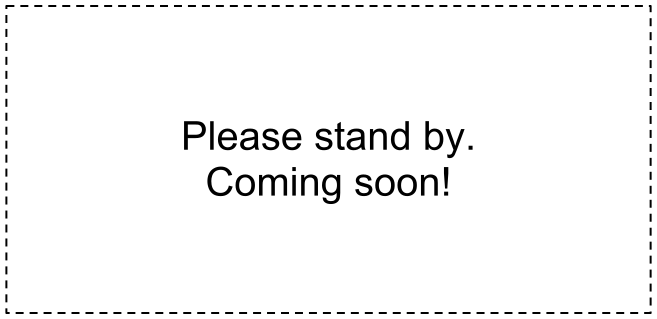
\includegraphics[width=\textwidth]{Images/dummy}
\caption{XBee prototyping interfaces}
\label{fig:xbee_prototyping_interfaces}
\end{figure}

The wireless software module uses an existing open-source software library to handle the low level communication with the XBee hardware, and adds an object oriented interface as well as utility classes that allow to use and control the wireless connection at a high abstraction level. More details on the design of the software module are given in section \ref{sec:wireless_communication_software}


\section{Base Station}
\begin{figure}[htb]
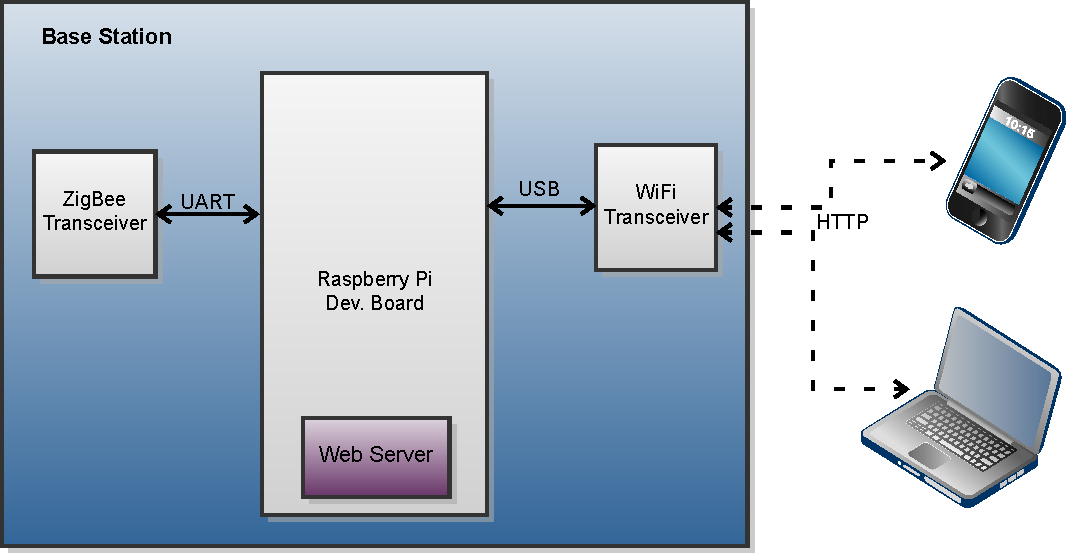
\includegraphics[width=\textwidth]{Images/BaseStationBlockDiagram}
\caption{Block Diagram: Base Station}
\label{fig:block_base_station}
\end{figure}

The base station collects data from the monitoring devices, stores this data in a database and makes it available and via a webserver running on the device itself. The advantage of using a website to provide access to the collected data is the support for a variety of devices with web access. In addition, it compensates disadvantage of the short range low data-rate ZigBee connection making the data accessible from anywhere.  


\subsection{Hardware platform}
The base station acts as a bridge between the “proprietary” monitoring stations and the end user, who wants an easy way to access the data that is collected by the system. The challenges for the base station lay mainly in the software domain. The only requirements that exist for the platform is that it has a to be able to interface an XBee device, a WLAN transceiver and provide means for mass data storage. 

For these reasons the decision was made, that an existing hardware platform would be used to implement the base station. The choice fell on the Raspberry Pi which provides a number of positive implications that are listed in table \ref{tab:raspberry_capabilities}.


\subsection{Raspberry Pi}
\begin{table}
\centering
\begin{tabular}{|l|m{6cm}|}
\hline
	Price &
	35£   \\ 
\hline
  	Software &
  	Raspberry can run a Debian based distribution, which gives access to a huge set of open-source programs and libraries  \\ 
\hline
	Connectivity &
	Features an ethernet port, USB host capabilities and HDMI output that could be used to attach a display to the base station  \\ 
\hline
	Extendability / GPIP  &
	20 GPIO pins, support for I2C, SPI, Serial  \\ 
\hline
	Storage &
	SD-Card slot with support for cards up to 64GB  \\ 
\hline
	Power consumption &
	Very low, between 1.5 and 2 Watt \\ 
\hline
 	Size &
 	Very small form factor (85.6mm x 56mm)  \\ 
\hline 
\end{tabular} 
\caption{Raspberry Pi capabilities}
\label{tab:raspberry_capabilities}
\end{table}

In summary it can be said that the Raspberry Pi is very well suited for rapid development of embedded systems, as long as they are not supposed to run on battery. It offers the convenience of developing software in a Linux environment while giving direct access to low level I/O capabilities for interfacing custom hardware.

\subsection{XBee}
As mentioned in section \ref{sec:wireless_connection} we use of XBee devices to implement the ZigBee network for data transmission between monitoring devices and the base station. These devices are widely-used in (homebrew) electronic projects, and they have the advantage that a Raspberry compatible XBee adapter board already exists. The adapter goes by the name of Slice of Pi and is shown in figure \ref{fig:xbee_prototyping_interfaces}.
